\documentclass[11pt]{article}
\usepackage{amsmath}
\usepackage{listings}
\usepackage{parskip}	%to remove paragraph indentation
\usepackage{float}	%to fix the image position

%Gummi|065|=)
\title{\textbf{Statistical Methods for Bioinformatics [I0U31a] \\Assignment 04 - Chapter 7}}
\author{Hamed Borhani}
\date{\today}
\usepackage{graphicx}
\begin{document}
\lstset{language=R, breaklines=true, basicstyle=\footnotesize} 

\maketitle

\newpage
\paragraph{7.9.1 }

\subparagraph{(a)}
When $x\leq\xi$ , then $(x - \xi)_{+} = 0$ and the coefficients are: $a_{1} = \beta_{0}$, $b_{1} = \beta_{1}$, $c_{1} = \beta_{2}$ and $d_{1} = \beta_{3}$

\subparagraph{(b)}
when $x>\xi$ , then $f(x) = \beta_0 + \beta_1x + \beta_2x^2 + \beta_3x^3 + \beta_4(x-\xi)^3$
\\so we have to expand the $\beta_4(x-\xi)^3$ to find $a_2, b_2, c_2$ and $d_2$ :
\begin{align*}
f(x) &= \beta_0 + \beta_1x + \beta_2x^2 + \beta_3x^3 + \beta_4(x-\xi)^3
\\&= \beta_0 + \beta_1x + \beta_2x^2 + \beta_3x^3 + \beta_4(x^3 - 3x^2\xi + 3x\xi^2 - \xi^3)
\\&= (\beta_0 -\beta_4\xi^3) + (\beta_1 + 3\beta_4\xi^2)x + (\beta_2 - 3\beta_4\xi)x^2 + (\beta_3 + \beta_4)x^3
\end{align*}
Therefore :
\begin{align*}
a_2 &= \beta_0 -\beta_4\xi^3
\\b_2 &= \beta_1 + 3\beta_4\xi^2
\\c_2 &= \beta_2 - 3\beta_4\xi
\\d_2 &= \beta_3 + \beta_4
\end{align*}

\subparagraph{(c)}
To show that a (piecewise)function is continuous at a point, one should show that two pieces are equal at that point:
\begin{align*}
f_1(x = \xi) &= \beta_0 + \beta_1\xi + \beta_2\xi^2 + \beta_3\xi^3\\\\
f_2(x = \xi) &= (\beta_0 -\beta_4\xi^3) + (\beta_1 + 3\beta_4\xi^2)\xi + (\beta_2 - 3\beta_4\xi)\xi^2 + (\beta_3 + \beta_4)\xi^3\\
f_2(x = \xi) &= \beta_0 + \beta_1\xi + \beta_2\xi^2 + \beta_3\xi^3
\end{align*}
\begin{center}
So $f_1(\xi) = f_2(\xi)$
\end{center}

\subparagraph{(d)}
\begin{align*}
f'_1(x = \xi) &= \beta_1 + 2\beta_2\xi + 3\beta_3\xi^2\\\\
f'_2(x = \xi) &= \beta_1 + 3\beta_4\xi^2 + 2(\beta_2 - 3\beta_4\xi)\xi + 3(\beta_3 + \beta_4)\xi^2\\
f'_2(x = \xi) &= \beta_1 + 3\beta_4\xi^2 + 2\beta_2\xi - 6\beta_4\xi + 3\beta_3\xi^2 + 3\beta_4\xi^2\\
f'_2(x = \xi) &= \beta_1 + 2\beta_2\xi + 3\beta_3\xi^2
\end{align*}
\begin{center}
So $f'_1(\xi) = f'_2(\xi)$
\end{center}

\subparagraph{(e)}
\begin{align*}
f''_1(x = \xi) &= 2\beta_2 + 6\beta_3\xi\\\\
f''_2(x = \xi) &= 6\beta_4\xi + 2\beta_2 - 12\beta_4\xi + 6\beta_3\xi + 6\beta_4\xi\\
f''_2(x = \xi) &= 2\beta_2 + 6\beta_3\xi
\end{align*}
\begin{center}
So $f''_1(\xi) = f''_2(\xi)$
\end{center}

\paragraph{7.9.9}
\subparagraph{(a)}
\subparagraph{(a)}
\begin{lstlisting}

library(MASS)

fit = lm(nox ~ poly(dis, 3), data = Boston)
\end{lstlisting}
\begin{lstlisting}[basicstyle = \ttfamily\footnotesize]
>summary(fit)
Call:
lm(formula = nox ~ poly(dis, 3), data = Boston)

Residuals:
      Min        1Q    Median        3Q       Max 
-0.121130 -0.040619 -0.009738  0.023385  0.194904 

Coefficients:
               Estimate Std. Error t value Pr(>|t|)    
(Intercept)    0.554695   0.002759 201.021  < 2e-16 ***
poly(dis, 3)1 -2.003096   0.062071 -32.271  < 2e-16 ***
poly(dis, 3)2  0.856330   0.062071  13.796  < 2e-16 ***
poly(dis, 3)3 -0.318049   0.062071  -5.124 4.27e-07 ***
---
Signif. codes:  0 ‘***’ 0.001 ‘**’ 0.01 ‘*’ 0.05 ‘.’ 0.1 ‘ ’ 1

Residual standard error: 0.06207 on 502 degrees of freedom
Multiple R-squared:  0.7148,	Adjusted R-squared:  0.7131 
F-statistic: 419.3 on 3 and 502 DF,  p-value: < 2.2e-16
\end{lstlisting}

\begin{figure}[H]
\centering
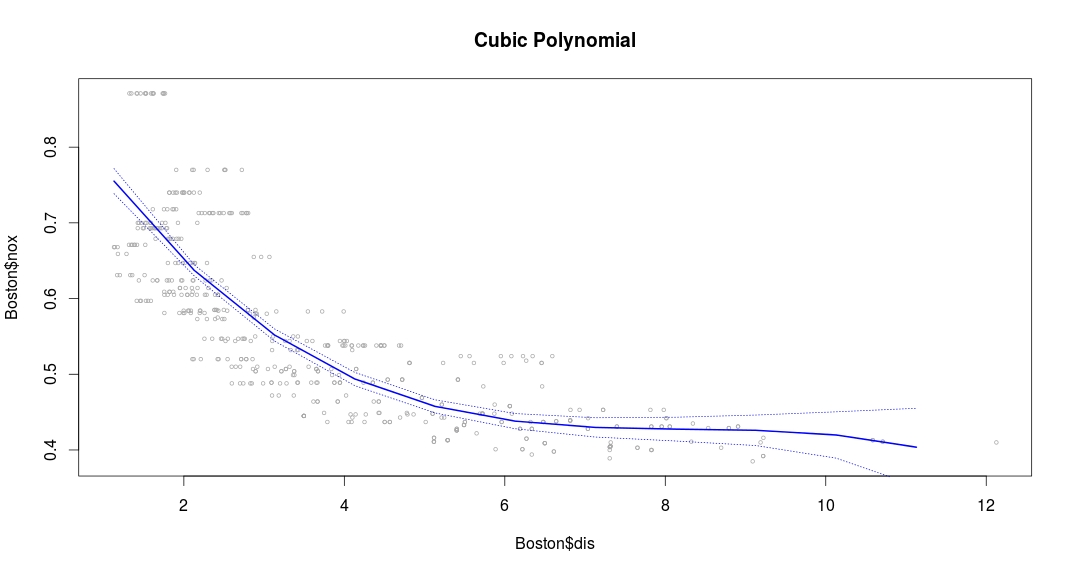
\includegraphics[scale=0.35]{/home/hamed/KUL/SEM2/stat/Rob/Labs+exercises/ex04_ch07/cubic.jpeg}
\caption{Cubic polynomial}
\end{figure}

\subparagraph{(b)}
\subparagraph{(b)}
\begin{lstlisting}
fit.1 = lm(nox ~ poly(dis, 1), data = Boston)
fit.2 = lm(nox ~ poly(dis, 2), data = Boston)
fit.3 = lm(nox ~ poly(dis, 3), data = Boston)
fit.4 = lm(nox ~ poly(dis, 4), data = Boston)
fit.5 = lm(nox ~ poly(dis, 5), data = Boston)
fit.6 = lm(nox ~ poly(dis, 6), data = Boston)
fit.7 = lm(nox ~ poly(dis, 7), data = Boston)
fit.8 = lm(nox ~ poly(dis, 8), data = Boston)
fit.9 = lm(nox ~ poly(dis, 9), data = Boston)
fit.10 = lm(nox ~ poly(dis, 10), data = Boston)
\end{lstlisting}

\begin{lstlisting}[basicstyle = \ttfamily\footnotesize]
>sum(fit.1$residuals^2)
[1] 2.768563
 sum(fit.2$residuals^2)
[1] 2.035262
> sum(fit.3$residuals^2)
[1] 1.934107
> sum(fit.4$residuals^2)
[1] 1.932981
> sum(fit.5$residuals^2)
[1] 1.91529
> sum(fit.6$residuals^2)
[1] 1.878257
> sum(fit.7$residuals^2)
[1] 1.849484
> sum(fit.8$residuals^2)
[1] 1.83563
> sum(fit.9$residuals^2)
[1] 1.833331
> sum(fit.10$residuals^2)
[1] 1.832171
\end{lstlisting}

\subparagraph{(c)}
Choosing the best polynomial degree based on Anova:

\begin{lstlisting}[basicstyle = \ttfamily\footnotesize]
> anova(fit.1, fit.2, fit.3, fit.4, fit.5, fit.6, fit.7, fit.8, fit.9, fit.10)
Analysis of Variance Table

Model  1: nox ~ poly(dis, 1)
Model  2: nox ~ poly(dis, 2)
Model  3: nox ~ poly(dis, 3)
Model  4: nox ~ poly(dis, 4)
Model  5: nox ~ poly(dis, 5)
Model  6: nox ~ poly(dis, 6)
Model  7: nox ~ poly(dis, 7)
Model  8: nox ~ poly(dis, 8)
Model  9: nox ~ poly(dis, 9)
Model 10: nox ~ poly(dis, 10)
   Res.Df    RSS Df Sum of Sq        F    Pr(>F)    
1     504 2.7686                                    
2     503 2.0353  1   0.73330 198.1169 < 2.2e-16 ***
3     502 1.9341  1   0.10116  27.3292 2.535e-07 ***
4     501 1.9330  1   0.00113   0.3040  0.581606    
5     500 1.9153  1   0.01769   4.7797  0.029265 *  
6     499 1.8783  1   0.03703  10.0052  0.001657 ** 
7     498 1.8495  1   0.02877   7.7738  0.005505 ** 
8     497 1.8356  1   0.01385   3.7429  0.053601 .  
9     496 1.8333  1   0.00230   0.6211  0.431019    
10    495 1.8322  1   0.00116   0.3133  0.575908    
---
Signif. codes:  0 ‘***’ 0.001 ‘**’ 0.01 ‘*’ 0.05 ‘.’ 0.1 ‘ ’ 1
\end{lstlisting}
P-values are significantly low while comparing Model1 (linear) to Model2 (quadratic) and Model2 (quadratic) to Model3 (cubic). But in comparing Model3 (cubic) to Model4 (quartic), p-value is not significantly low, therefore a cubic polynomial fit sounds a good fit.

\subparagraph{(d)}
\subparagraph{(d)}
\begin{lstlisting}
library(splines)

fit <- lm(nox ~ bs(dis, df = 4), data = Boston)
pred <- predict(fit, newdata = list(dis = dis.grid), se = T)
plot(Boston$dis, Boston$nox, col = "grey")
lines(dis.grid, pred$fit, lwd = 2, col = "blue")
lines(dis.grid, pred$fit + 2*pred$se.fit, lty = "dashed")
lines(dis.grid, pred$fit - 2*pred$se.fit, lty = "dashed")
\end{lstlisting}

\begin{figure}[H]
\centering
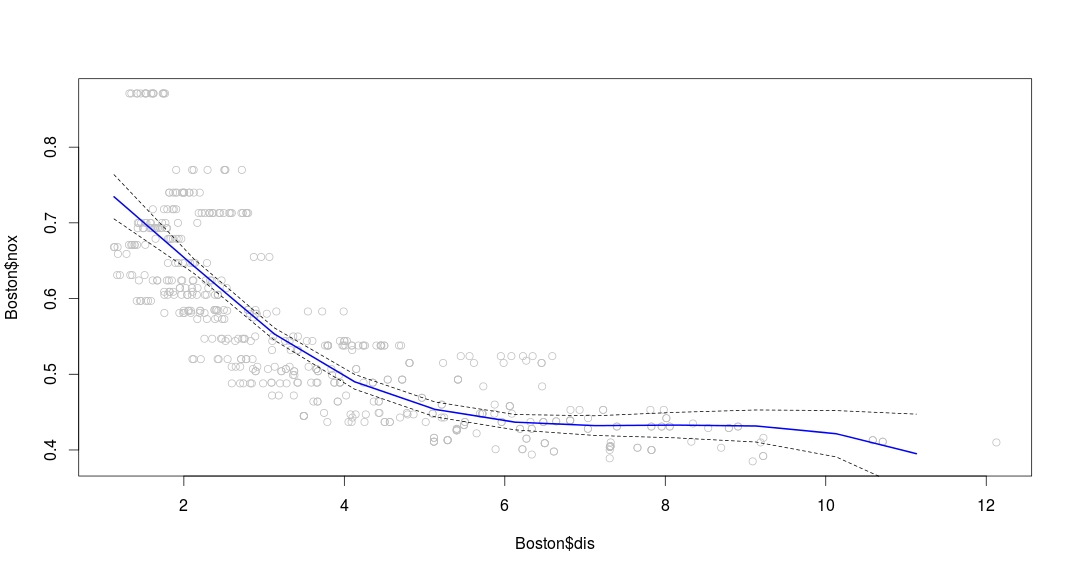
\includegraphics[scale=0.35]{/home/hamed/KUL/SEM2/stat/Rob/Labs+exercises/ex04_ch07/spline.jpeg}
\caption{Spline fit with uniform knots}
\end{figure}
(Knots were chosen uniformly)
\subparagraph{(e)}
\subparagraph{(f)}
\end{document}
